\apendice{Documentación técnica de programación}


\section{Introducción}

En este apéndice se van a describir todos aquellos aspectos que se consideren de interés para una persona que desee continuar el desarrollo del proyecto o quiera obtener un conocimiento más avanzado del mismo.

\section{Estructura de directorios}

A continuación se va a hacer mención a la funcionalidad de cada una de las carpetas que conforman el árbol de directorios de nuestro proyecto:

\begin{itemize}
	\item \textbf{src:} Carpeta destinada a almacenar el código fuente la aplicación.
	\begin{itemize}
		\item \textbf{main/scala:} Este directorio contendrá todos los ficheros fuente cuya ejecución forme parte del proyecto final y estén escritos en Scala. Al no haberse usado ningún otro lenguaje ni contar con clases para realizar pruebas, este es el único directorio de la carpeta ``src''.
	\end{itemize}
	\item \textbf{resources:} Carpeta destinada a contener todos aquellos elementos que, sin ser código, también son necesarios para la ejecución del programa. Aquí podríamos incluir fichero .xml, html, imágenes o cualquier otro fichero multimedia, etc.
	\begin{itemize}
		\item \textbf{gui:} Contiene todos los recursos utilizados por la interfaz gráfica.
		\item \textbf{loggerStrings:} Almacena ficheros de texto con sentencias que pueden ser utilizadas por los diferentes \textit{logger} en diferentes clases de nuestro programa.
	\end{itemize}
	\item \textbf{target:} Contiene los archivos resultantes de aplicar alguna operación de Maven sobre el proyecto (compilación, empaquetado o generación de documentación). Para más información al respecto visitar la sección \ref{subsec:compilacion} y \ref{subsec:documentacion}.
	\begin{itemize}
		\item \textbf{site/scaladocs:} Ruta que contiene la documentación del proyecto generada por Scaladoc.
	\end{itemize}
\end{itemize}


\section{Manual del programador}

A lo largo de esta sección vamos a describir diferentes tareas que, pese a no tener 
relación directa con la ejecución del programa, pueden conducir a un manejo más avanzado del mismo o a poder acceder a valores de la ejecución en los que un usuario normal no está interesado.

Antes de proceder es necesario comprender y haber realizado el proceso de instalación de todos los componentes mencionados en la sección \ref{sec:Instalacion}, independientemente de si esos componentes han sido marcados como opcionales o no para el usuario normal.

\subsection{Configurando Spark para guardar información sobre ejecuciones}\label{subsec:configurandoSpark}

Con la configuración por defecto, Spark apenas almacena información sobre las ejecuciones realizadas, pudiendo acceder a las mediciones solo mientras el programa se está ejecutando. A lo largo de esta sección explicaremos que es posible modificar este comportamiento y la manera de lograrlo.

Lo primero que necesitamos es modificar algunas propiedades de Spark. En su carpeta de configuración  (\textit{\$SPARK\_HOME/conf}) debemos buscar un fichero por nombre ``spark-defaults.conf''. Si es la primera vez que realizamos este tipo de operaciones es posible que este fichero no exista, haciendo necesario crearlo nosotros mismos o renombrar el fichero ``spark-defaults.conf.template'' que actúa de ejemplo y está situado en la misma carpeta.

Sea cual sea la opción elegida, en nuestro fichero de configuración ``spark-defaults.conf'' escribiremos las siguientes líneas:

\begin{lstlisting}[basicstyle=\small]
spark.eventLog.enabled	true
spark.eventLog.dir	    /opt/spark-1.5.1/logs/exec-logs
spark.history.fs.logDirectory /opt/spark-1.5.1/logs/exec-logs
\end{lstlisting}

La primera línea es obligatoria y no admite cambios. Las dos siguientes sirven para indicar el fichero donde deseamos almacenar la información de las ejecuciones. La ruta seleccionada es indiferente, pero es necesario destacar dos aspectos:
\begin{itemize}
\item Las rutas dos rutas indicadas han de ser iguales.
\item Las rutas han de apuntar a un directorio existente. Si indicamos una ruta inexistente Spark no generará los directorios que falten, sino que emitirá un error cuando intentemos ejecutar una aplicación y esta quiera guardar sus datos de ejecución. Es por ello que, en el caso concreto de la configuración ofrecida como ejemplo, deberíamos crear la carpeta ``exec-logs'' en  \textit{/opt/spark-1.5.1/logs} antes de proceder.
\end{itemize}

Con esto, deberíamos contar con toda la información de nuestras ejecuciones aun después de que estas hayan acabado. En la siguiente sección, \ref{subsec:monitorizacion}, hablaremos de como acceder a todos estos datos para su posterior análisis.


\subsection{Monitorización y análisis}\label{subsec:monitorizacion}

Un aspecto clave en el desarrollo de aplicaciones para \textit{big data} es el de controlar y analizar el rendimiento de los algoritmos. Para ello, vamos a explicar en la siguiente sección como acceder a este tipo de información. No es objetivo de este anexo, sin embargo, explicar toda la información analizable ni la manera en la que ésta se organiza.

Antes de continuar, es necesario indicar que toda esta información proporcionada aquí corresponde a la manera de analizar una aplicación ejecutada en el modo \textit{Standalone} de Spark (ver sección \ref{subsec:modosDespliegueSpark} para más información). Si Spark se ejecutase usando algún administrador de clústeres el modo de acceder a la información podría ser distinto dependiendo del software usado. Igualmente, si ejecutamos en modo local no existe una manera de acceder a los datos de análisis una vez la aplicación ha finalizado su ejecución.

Con todo, comenzaremos contemplando la posibilidad de observar la ejecución de un programa mientras éste está todavía en ejecución. Esto puede hacerse accediendo, mediante el navegador, a la ruta \url{http://localhost:4040} (suponemos que nuestra máquina es el nodo maestro). Podemos ver un ejemplo de la página inicial en la imagen \ref{fig:img/anexo/pantalla_4040}. Esta información solo estará disponible mientras la aplicación lanzada siga ejecutando, y toda la información que podemos ver será borrada si no hemos seguido los pasos descritos en la sección \ref{subsec:configurandoSpark}.

\imagen{img/anexo/pantalla_4040}{Ejemplo de monitorización de una aplicación en marcha.}

Suponiendo que queremos realizar un análisis de todas las aplicaciones que han sido lanzadas en la red de nodos en modo \textit{Standalone}, podemos hacerlo consultado la dirección \url{http://localhost:8080}. Además de información referente a nuestro clúster, podemos observar un listado de aplicaciones ejecutadas o en ejecución, a cuya información se puede acceder pulsando sobre cualquiera de ellas (ver imagen \ref{fig:img/anexo/pantalla_8080}).

\imagen{img/anexo/pantalla_8080}{Pantalla de inicio de un clúster Standalone.}

De nuevo, la ruta indicada ruta es válida si únicamente estamos trabajando en la máquina local o somos el nodo maestro de la red. Igualmente, volvemos a recordar que hemos tenido que habilitar la opción de Spark para guardar información de las ejecuciones, tal y como se describe en \ref{subsec:configurandoSpark}.

Por último, si deseamos acceder a toda la información de ejecuciones guardada en nuestra máquina, podemos acceder iniciando el servicio ``History Server'' y accediendo a la ruta (\url{http://localhost:18080/}), donde se nos mostrará un listado con todas las aplicaciones ejecutadas de las que se tiene información. Para iniciar el servicio mencionado, desde consola de comandos, debemos escribir el comando:

\begin{lstlisting}[language=bash]
$ $SPARK_HOME/sbin/start-history-server.sh
\end{lstlisting}

Podemos ver un ejemplo del histórico de ejecuciones en la imagen \ref{fig:img/anexo/pantalla_18080}.

\imagen{img/anexo/pantalla_18080}{Ejemplo de monitorización de una aplicación en marcha.}


\todo{Monitorización y análisis usando Google Dataproc??????}

\section{Compilación, instalación y ejecución del proyecto}

A lo largo de esta sección vamos a hablar de todos los pasos necesarios para poder trabajar sobre el código del proyecto. Esto incluye la instalación de diferentes componentes, la configuración del entorno de desarrollo y la comprensión de la herramienta Apache Maven como administrador de las labores como la compilación.

\subsection{Instalación}

Si deseamos trabajar sobre el código del proyecto, además de necesitar todos los materiales definidos en la sección \ref{sec:Instalacion} vamos a necesitar los definidos en este apartado.

\subsubsection{Scala 2.11.7}
Aunque podemos descargar la última versión de Scala desde la página oficial (\url{http://www.scala-lang.org/}). La descarga que se nos ofrece por defecto es un archivo .tar.gz que nos obligaría a realizar toda la instalación manualmente (suponiendo que estamos en un sistema Ubuntu como el utilizado durante el proyecto).

Por ello, vamos a realizar la instalación mediante un archivo .deb (paquete Debian) que también puede ser utilizado por nuestro sistema y que nos ahorrará realizar la instalación manualmente. Podemos acceder al repositorio que guarda este paquete desde un navegador (\url{http://www.scala-lang.org/files/archive/}) o descargarlo mediante el siguiente comando:

\begin{lstlisting}[language=bash]
$ wget www.scala-lang.org/files/archive/scala-2.11.7.deb
\end{lstlisting}

Independientemente del método seguido, una vez tengamos el archivo en nuestro ordenador ejecutamos el siguiente comando desde la carpeta que contenga el paquete .deb:

\begin{lstlisting}[language=bash]
$ sudo dpkg -i scala-2.11.7.deb
\end{lstlisting}

Si todo ha salido correctamente, una vez termine de ejecutarse la orden anterior podemos ejecutar el comando \textit{scala -version} y esperar una salida similar a esta:

\begin{lstlisting}[language=bash]
$ scala -version
Scala code runner version 2.11.7 -- Copyright 2002-2013
\end{lstlisting}

Recordar que, en el caso de utilizar cualquier otra versión de Scala, esta tiene que ser compatible con la versión Java que se encuentre instalada. Por ejemplo, Java 8 solo puede ser utilizado a partir de versiones 2.11 y será obligatorio a partir de la versión de Scala 2.12. \cite{Scala2.12Roadmap}

\subsubsection{Scala IDE}

Scala IDE es el entorno de desarrollo utilizado durante el proyecto.

Descargaremos la  última versión disponible del producto desde su página oficial: \url{http://scala-ide.org/}

Dentro de las posibles descargas que podemos seleccionar, elegiremos aquella que esté destinada a nuestro sistema operativo, en nuestro caso concreto, ``Linux - 64 bits''. Al descargar esta herramienta, en realidad estamos descargando el entorno de desarrollo Eclipse (\url{https://eclipse.org/}) con una serie de \textit{plugins} añadidos, entre los que destaca el llamado Scala IDE.

Una vez descargado, descomprimiremos el archivo en la ruta \textit{/opt}. Mediante línea de comandos podemos hacerlo utilizando la siguiente sentencia:

\begin{lstlisting}
$ cd /opt/ && sudo tar -zxvf \
~/Downloads/scala-SDK-4.2.0-vfinal-2.11-\
linux.gtk.x86_64.tar.gz
\end{lstlisting}

Recuerde que el código puede cambiar dependiendo del nombre del archivo que sea descargado o del directorio donde se encuentre.

\subsection{Importando el proyecto en Scala IDE}


Suponiendo que se ha seguido la instalación del entorno de desarrollo mencionado (Scala IDE) seguiremos los siguientes pasos para importar y ejecutar nuestro proyecto desde el propio programa.

Primero de todo, para importar el código a nuestro lugar de trabajo, debemos dirigirnos al menú superior, opción ``File'' y, de entre las opciones del menú desplegable, seleccionar ``Import''. Alternativamente también podemos realizar la misma operación haciendo clic derecho sobre el panel de nombre ``Package explorer''.

Veremos un nuevo diálogo similar al mostrado en la figura \ref{fig:img/anexo/existing_maven_projects}, donde seleccionaremos, entre todas las opciones, aquella que diga ``Existing Maven Projects''. Posteriormente, presionamos sobre el botón continuar.

\imagen{img/anexo/existing_maven_projects}{Diálogo para seleccionar un médoto de importación en Eclipse IDE.}

En el nuevo diálogo presionaremos sobre el botón ``Browse'' para indicar el directorio principal de nuestro proyecto. Si todo es correcto, el resultado debería ser similar al mostrado en la imagen \ref{fig:img/anexo/proyecto_importado}.

\imagen{img/anexo/proyecto_importado}{Diálogo para importar un projecto al entorno Eclipse IDE.}

Pulsamos sobre el botón aceptar y, si todo ha salido correctamente, deberíamos poder ver nuestro proyecto en el menú lateral izquierdo, tal como muestra \ref{fig:img/anexo/paquete_importado}

\imagen{img/anexo/paquete_importado}{Paquete importado en el menú lateral.}


\subsection{Ejecutando el proyecto en Scala IDE}

Como puede observarse en el manual del usuario (\ref{sec:manualUsuario}) el lanzamiento de una aplicación en Spark se realiza mediante un script que proporciona el propio Spark y en el cual se pueden indicar ciertos parámetros de ejecución. Por ello, para el lanzamiento del programa desde Eclipse hemos de modificar añadir algún fragmento de código que genere una configuración de Spark que, en cualquier otro método de lanzamiento, es creada por el script utilizado.

Para ello hemos de modificar un fragmento de código en la clase \textit{ISClassExec} del paquete \textit{launcher.execution}, tal y como puede verse en \ref{lst:codigoSpark} y \ref{lst:codigoEclipse}


\begin{lstlisting}[language=Java,tabsize=4,frame = single,caption=Código para la ejecución del programa mediante el script ``spark-sumbit''. ,captionpos=b,label=lst:codigoSpark]
val sc = new SparkContext()
\end{lstlisting}

\begin{lstlisting}[language=Java,tabsize=4,frame = single,caption=Ejemplo de código para la ejecución del programa desde Eclipse. ,captionpos=b,label=lst:codigoEclipse]
	val master = "local[2]"
    val sparkConf =
  	  new SparkConf().setMaster(master)
  	  .setAppName("Prueba_Eclipse")
    val sc = new SparkContext(sparkConf)
\end{lstlisting}

Ahora, debemos indicar de manera manual cual será la clase principal que deseamos lanzar. Es posible que esto cambie de acuerdo al tipo de ejecución que queremos realizar (lanzar la interfaz gráfica o un experimento de Spark), pero los pasos a seguir son idénticos.

Desde la pantalla de Scala IDE nos dirigiremos al menú superior, presionamos sobre ``Run'' y seleccionamos la opción ``Run configurations''. Esto abrirá una nueva ventana similar a la mostrada en la figura \ref{fig:img/anexo/run_configurations}.

Presionando dos veces sobre el texto ``Scala application'' podremos generar una nueva configuración para el proyecto. Allí rellenaremos los campos requeridos, con especial interés al campo ``Main Class'', que deberá escribirse manualmente porque el entorno no detecta ninguna de las clases principales de los proyectos. En nuestro caso, ese campo siempre será ``launcher.ExperimentLauncher'' para lanzar experimentos y ``gui.SparkISGUI'' para lanzar la interfaz gráfica.


\imagen{img/anexo/run_configurations}{Ventana de configuración de ejecuciones en Scala IDE.}


Finalmente, si deseamos introducir argumentos al iniciar una ejecución, podemos hacerlo desde la pestaña ``Arguments'', en la ventana anterior, rellenando el campo ``Program arguments'' con la información que deseemos (ver ejemplo en \ref{fig:img/anexo/arguments_configuration})

\imagen{img/anexo/arguments_configuration}{Ventana de configuración de ejecuciones en Scala IDE - Argumentos.}


Con todo definido, podemos presionar sobre el botón ``Run'' para comenzar a ejecutar nuestro programa.

Para posteriores ejecuciones no necesitaremos volver a definir de nuevo todo el proceso, sino que la opción será guardada y podrá ser accedida de manera sencilla seleccionándola desde el menú desplegable que proporciona el botón de ejecutar en el menú superior de Eclipse (ver figura \ref{fig:img/anexo/menu_superior_eclipse}).

	\begin{figure}[!h]
		\centering
		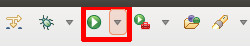
\includegraphics[width=0.4\textwidth]{img/anexo/menu_superior_eclipse}
		\caption{Fragmento del menú superior de Scala IDE.}\label{fig:img/anexo/menu_superior_eclipse}
	\end{figure}
	
	
	\subsection{Compilación}\label{subsec:compilacion}

Para realizar la labor de compilación vamos a necesitar del software Apache Maven, cuya instalación ha sido indicada en \ref{subsec:instalaMaven}. Una vez contemos con este requisito la operación será prácticamente automática.

Desde consola nos dirigimos al directorio raíz donde esté situado el proyecto. Una vez allí, ejecutamos el comando siguiente:

\begin{lstlisting}[language=bash]
$ mvn clean package
\end{lstlisting}

Si es la primera vez que se realiza esta operación sobre el proyecto, o incluso la primera vez que se utiliza Maven, es muy probable que se requiera de algo de tiempo adicional mientras se descargan todos los materiales necesarios para poder llevar a cabo la labor de compilación.

Toda la información referente a la administración del proyecto (dependencias, fases, etc.) debe encontrarse en el documento situado en la carpeta raiz. El nombre de este documento suele ser ``pom.xml'' pero, dado que en este proyecto existen diferentes distribuciones finales y, por norma, un fichero de este tipo solo debería generar una única distribución, si deseamos utilizar cualquier otro fichero de los proporcionados para administrar el proceso deberemos ejecutar el comando:

\begin{lstlisting}[language=bash]
$ mvn -f otro_pom clean package
\end{lstlisting}

Actualmente se cuentan con los siguientes ficheros para generar distribuciones:
\begin{itemize}
\item \textbf{pom.xml:} Realiza una compilación y empaquetado de todo el material del proyecto. Debe encontrarse instalada la versión de Scala 2.11 para realizar la compilación.
\item \textbf{pom\_gui:} Genera una distribución que contará únicamente con los componentes gráficos del sistema. Vuelve a ser requerido Scala 2.11 para la fase de compilación.
\item \textbf{pom\_cluster:} Crea una distribución que contendrá todos los elementos menos los relacionados con la interfaz gráfica. La compilación ha de realizarse esta vez con Scala 2.10.
\end{itemize}

\subsection{Generando documentación}\label{subsec:documentacion}

De nuevo mediante el uso de Apache Maven, podemos realizar labores de documentación del código del proyecto utilizando el siguiente comando desde el directorio raíz del proyecto:

\begin{lstlisting}[language=bash]
$ mvn scala:doc@Scaladoc
\end{lstlisting}

La documentación será generada en la carpeta \textit{target/sites/scaladocs} utilizando el software ``Scaladoc''.

Es necesario indicar que este generador de documentación tiene algunos inconvenientes:
\begin{itemize}
\item En primer lugar, ignora cualquier variable, método o clase privada, sin la posibilidad de poder revertir esta opción. Es por ello que cualquier material marcado como privado no aparecerá en los documentos generados.
\item En segundo lugar, el material generado mostrará todos los métodos de una clase, los definidos y los heredados de cualquier otro componente, aunque no pertenezca a nuestra librería. Esto puede llegar a resultar molesto en algunas clases, como las pertenecientes a la interfaz gráfica, y es una opción que, de nuevo, no puede modificarse. En este caso, podemos presionar sobre el botón ``Hide all'' que encontraremos en cada clase y que permite ocultar todos aquellos métodos o atributos heredados de componentes que, por lo general, no suelen interesarnos.
\end{itemize}
 

\imagen{img/anexo/scaladoc}{Página principal de la documentación con Scaladoc}

\section{Otros aspectos relevantes a la hora de implementar}
Por parte del programador, es necesario conocer una serie de aspectos que han influido en la implementación actual del código y que podrían seguir siendo influyentes si se continuase el trabajo.

\subsection{Versión de Scala}

Uno de los problemas a los que se enfrenta este proyecto se encuentra con la versión de Scala utilizada para compilar las clases. Scala 2.10 y Scala 2.11 no producen binarios compatibles, lo que impide que programas escritos en la versión anterior puedan ser leídos cuando esperamos clases compiladas para Scala 2.11 y viceversa.

Se comenzó el proyecto utilizando la versión de Scala 2.11 y, por lo tanto, se configuró Spark para trabajar con esa misma versión. Sin embargo, nos hemos encontrado con la necesidad de ejecutar el proyecto en sistemas donde Spark continua utilizando Scala 2.10.

Este cambio de versiones, además de afectar a la manera en la que debemos compilar el proyecto, tiene influencia a la hora de programar, pues podemos encontrar clases que cumplan su función en una versión y resulten en algún error en la siguiente. 

Pensemos, por ejemplo, en la clase \textit{scala.util.Random}, cuya versión en Scala 2.10 no es serializable, mientras que en su versión siguiente sí lo es. Esto hace que, en caso de querer distribuir dicha clase entre un grupo de nodos, la acción resulte en error con versiones anteriores a Scala 2.11. En este caso concreto, se ha suprimido el uso de la clase \textit{scala.util.Random} para ser sustituido por \textit{java.util.Random}, que no presenta este tipo de problemas.

No se han encontrado más clases que ocasionen errores de compatibilidad pero se advierte este problema como medida de precaución para futuras iteraciones.


\subsection{k-folds cross-validation}

Uno de los problemas que ya hemos mencionado anteriormente tanto en otros anexos como en la propia memoria, es que Spark todavía se encuentra en un estado inicial donde algunos de los recursos que proporciona son escasos.

Quiero destacar el caso de la función \textit{kfolds}que podemos encontrarnos en la clase \textit{org.apache.spark.mllib.util.MLUtils} de la librería de Spark. Esta función, en la versión que hemos trabajado con Spark, se encuentra en estado ``experimental'' según la propia documentación de la clase \cite{SparkMLUtils}.

Se ha probado y demostrado durante este proyecto que la implementación actual de este método dista mucho de la implementación en Weka, la alternativa secuencial a Spark que hemos utilizado en este proyecto. Los \textit{k}-folds generados por Spark dividen el subconjunto inicial de tal manera que el resultado de clasificación final de nuestros experimentos se ve gravemente perjudicado. Se atribuye esto a que la función en Spark no realiza divisiones estratificadas, esto es, divisiones donde la proporción de un determinado tipo de instancias en el subconjunto final es similar a su proporcion en el conjunto completo.

Como la finalidad de este proyecto no ha sido la de profundizar sobre este aspecto, se ha implementado una manera crear los kfolds utilizando otras operaciones de Spark (función ``sample'' de la estructuras RDD ) y algunas operaciones sobre conjuntos. Si bien la solución aportada parece haber resuelto el problema, es necesario indicar que genera problemas en conjuntos de datos donde las instancias recogidas están repetidas muchas veces dentro del conjunto de datos.

Por todo esto, se anima al futuro programador a comprobar el funcionamiento de la función \textit{kfolds} que proporcione Spark o a tener en cuenta las limitaciones de la implementación proporcionada.

\subsection{Medición de tiempos de filtrado usando ISClassExecTest} \label{subsec:ISClassExecTest}

Puede ser de interés para el programador conocer la razón por la cual la clase \textit{launcher.execution.ISClassExecTest}, destinada a medir el tiempo de ejecución de la selección de instancias, posee una serie de operaciones que no se encuentran incluidas en la versión principal (\textit{launcher.execution.ISClassExec}).

Consideremos el siguiente fragmento de código, encargado de realizar la medición del tiempo que tardamos en filtrar un conjunto de datos de nombre ``train''


\begin{lstlisting}[language=Java,tabsize=4,frame = single,caption=Código de medición de tiempo de filtrado ,captionpos=b,label=lst:codigoEclipse]
    train.persist()
    train.name = "TrainData"
    train.foreachPartition { x => None }

    // Instanciamos y utilizamos el selector de instancias
    val start = System.currentTimeMillis
    val resultInstSelector = applyInstSelector(instSelector, train, sc).persist
    resultInstSelector.foreachPartition { x => None }
    executionTimes += System.currentTimeMillis - start
\end{lstlisting}

Pueden observarse varias cosas que no vemos en una ejecución normal:
\begin{itemize}
	\item El conjunto de datos ``train'' se persiste antes de iniciar la medición. Esto se realiza para estar seguros de que, a la hora de medir los tiempos de ejecución, nuestro conjunto de datos estará distribuido completamente entre nuestros nodos.
	\item Se realizan una serie de operaciones sin aparente sentido, pues vemos hasta en dos ocasiones la sentencia \textit{foreachPartition \{ x $=>$ None \}} que, teóricamente, manda hacer ``nada'' a cada partición. En realidad, esta sentencia tiene como finalidad forzar a Spark a realizar todas las operaciones necesarias para calcular la estructura RDD sobre la que se está aplicando. Puede parecer un tema trivial pero eliminar la sentencia puede influir en las mediciones realizadas.
	
	Pondremos por ejemplo el algoritmo LSHIS. Este algoritmo persiste la estructura RDD que recibe cuando se le encomienda aplicar una selección de instancias, es decir, tiene definida una operación \textit{.persist} al início del método \textit{applyInstSelector}. A simple vista podemos pensar que esta operación ya está definida en el código que hemos proporcionado un par de párrafos más arriba y que, por lo tanto, será omitida por el organizador de tareas cuando lancemos el programa. Sin embargo, si no hemos utilizado primero la operación \textit{foreachPartition \{ x $=>$ None \}}, el efecto que conseguiremos no será el esperado y el tiempo de distribución de la estructura RDD a través de los nodos será tenido en cuenta en la medición, alqo que consideramos indeseable.
\end{itemize}


Es necesario comprender que la clase \textit{ISClassExecTest} fue creada con la intención de medir de la manera más precisa posible los tiempos de ejecución del filtrado en Spark. Sin embargo, en tareas de \textit{big data}, esto no es lo habitual, pues una precisión medida en milisegundos no tiene sentido cuando las ejecuciones pueden durar días. Es por ello que, para mediciones que no requieran gran precisión, podemos utilizar la información que presentan las herramientas de monitorización de Spark (ver \ref{subsec:monitorizacion}).
